\documentclass[9pt,twocolumn,twoside]{osajnl}
						
\usepackage{bbm}

\journal{josaa} % Choose journal (ao, ol, josaa, josab)

\setboolean{shortarticle}{false} % true = letter, false = research article

\title{Optical trimmer, \\ A theoretical physics approach to photonic lattices}

\author[1]{A. Stoffel}
\author[2,*]{B. M. Rodríguez-Lara}

\affil[1]{Instituto Nacional de Astrof\'{\i}sica, \'Optica y Electr\'onica, Calle Luis Enrique Erro No. 1, Sta. Ma. Tonantzintla, Pue. CP 72840, M\'exico}
\affil[2]{Instituto Nacional de Astrof\'{\i}sica, \'Optica y Electr\'onica, Calle Luis Enrique Erro No. 1, Sta. Ma. Tonantzintla, Pue. CP 72840, M\'exico}

\affil[*]{Corresponding author: bmlara@inaoep.mx}

\dates{Compiled \today}

\ociscodes{(050.5298) Photonic crystals; (230.4555) Coupled Resonators; (230.7370) Waveguides;  (350.5500) Propagation. \textcolor{red}{Is there any waveguide devices?}}

\doi{\url{http://dx.doi.org/10.1364/ao.XX.XXXXXX}}

\begin{abstract}
We study electromagnetic field propagation through a triangular array of identical waveguides using a symmetry based approach to take advantage of the underlying $SU(3)$ symmetry.

\end{abstract}

\setboolean{displaycopyright}{true}

\begin{document}

\maketitle
\thispagestyle{fancy}
\ifthenelse{\boolean{shortarticle}}{\abscontent}{}

%%%%%%%%%%%%%%%%%%%%%%%%%%%%%%%%%%%%%%%%%%%%%%%%%%%%%%%%%%%%%%%%%%%%%%%%%%%%%%%%%%%%%%%%%%%%%%%%%%%
% Introduction
%%%%%%%%%%%%%%%%%%%%%%%%%%%%%%%%%%%%%%%%%%%%%%%%%%%%%%%%%%%%%%%%%%%%%%%%%%%%%%%%%%%%%%%%%%%%%%%%%%%
\section{Introduction}

\textcolor{red}{Some random ideas that may help write a coherent introduction, in no particular order}

In chemistry, a trimer is composed of three identical building blocks, we can borrow such an idea and think of three coupled identical photonic waveguides as an optical trimer.

Passive planar three-waveguide couplers have proved a reliable platform for fast, robust beam coupling based on adiabatic coupling or Ermakov-Lewis-Riesenfeld invariants \cite{Schneider2001p129,Narevicius2005p3362,Tseng2013p2478,Paspalakis2006p30,Salandrino2009p4524,RodriguezLara2014p013802}.
 
The planar platform has been used in three-waveguide nonlinear directional couplers, where the waveguides present an active Kerr nonlinearity, to produce all-optical spatial switching \cite{Finlayson1990p2276,Stegeman1990p95,Artigas1996p53,Chen1997p287,Liu2003p2930,Khan2008p9417,Tao2011p071104} and logic gates \cite{Menezes2007p1191}.

Triangular three-waveguide nonlinear directional couplers have been used to design all-optical logic gates \cite{Menezes2007p107,Coelho2013p731}.

Light propagating through a three-waveguide coupler with can be described by coupled mode theory, c.f. \cite{RodriguezLara2015p068014} and references therein,
\begin{eqnarray}
-i \partial_{z} \mathcal{E}_{0}(z) &=& \omega_{0}(z) \mathcal{E}_{0}(z) +   g_{01}(z) \mathcal{E}_{1}(z) + g_{02}(z) \mathcal{E}_{2}(z), \\
 -i \partial_{z} \mathcal{E}_{1}(z) &=& \omega_{1}(z) \mathcal{E}_{1}(z) + g_{01}(z) \mathcal{E}_{0}(z) + g_{12}(z) \mathcal{E}_{2}(z), \\
 -i \partial_{z} \mathcal{E}_{2}(z) &=& \omega_{2}(z) \mathcal{E}_{2}(z) + g_{02}(z) \mathcal{E}_{0}(z) + g_{12}(z) \mathcal{E}_{1}(z),
\end{eqnarray}
where the complex field amplitude at the $j$th waveguide is given by $\mathcal{E}_{j}(z)$, the effective refractive index at the $j$th waveguide is $\omega_{j}(z)$, and the effective coupling between the $j$th and $k$th waveguides is $g_{jk}(z)$.
These complex field equations can be cast in a Schr\"odinger-like form \cite{RodriguezLara2015p068014},
\begin{eqnarray}
- i \partial_{z} \vert \mathcal{E}(z) \rangle = \hat{H}(z) \vert \mathcal{E}(z) \rangle,\label{eq:diff}
\end{eqnarray}
where kets from Dirac notation represent column vectors,
\begin{eqnarray}
\vert \mathcal{E}(z) \rangle = \left( \mathcal{E}_{0}(z), \mathcal{E}_{1}(z), \mathcal{E}_{2}(z) \right)^{T}, 
\end{eqnarray}
and operators represent square matrices, in this particular case, the mode-coupling matrix,
\begin{eqnarray}
\hat{H}(z) = \left( \begin{array}{ccc} 
\omega_{0}(z)  & g_{01}(z) & g_{02}(z) \\
g_{01}(z) & \omega_{1}(z) & g_{12}(z) \\
g_{02}(z) & g_{12}(z) & \omega_{2}(z)
\end{array} \right), \label{eq:hmlt}
\end{eqnarray}
points to an underlying $SU(3)$ symmetry.
For the sake of simplicity we will require a normalized total intensity, $\sum_{j} \vert \mathcal{E}_{j} \vert^2 =1$

%%%%%%%%%%%%%%%%%%%%%%%
%%%% DRAFT
%//////////////////////////////////////////////%//////

\section{Classical mechanics and envelopes}

In quantum mechanics, the Hamiltonian for three coupled harmonic oscillators, 
\begin{eqnarray}
	\hat{H}(t) = \sum_{j=0}^{2} \omega_j(t) \hat{a}^{\dagger}_j \hat{a}_{j} + \sum_{j\neq k=0}^{2} g_{jk}(t) \hat{a}^{\dagger}_j \hat{a}_k,
\end{eqnarray}
in the single photon limit,
\begin{eqnarray}
	\left\vert \psi(t) \right\rangle = \mathcal{E}_{0}(t) \left\vert 1, 0, 0 \right\rangle  +
	\mathcal{E}_{1}(t) \left\vert 0,1,0 \right\rangle + \mathcal{E}_{2}(t) \left\vert 0,0,1 \right\rangle,
\end{eqnarray}
with $ \sum_{j} \vert \mathcal{E}_{j}(z) \vert^2 = 1$, yields a differential equation set equivalent to the mode coupling theory result, Eq.(\ref{eq:ddiff}) up to substitution of backwards time by propagation distance,
\begin{eqnarray}
	i \partial_t	
	\left( \begin{array}{c} 
		\mathcal{E}_{0}(t) \\
		\mathcal{E}_{1}(t) \\
		\mathcal{E}_{2}(t)
	\end{array} \right) =
	\left( \begin{array}{ccc} 
		\omega_{0}(t)  & g_{01}(t) & g_{02}(t) \\
		g_{01}(t) & \omega_{1}(t) & g_{12}(t) \\
		g_{02}(t) & g_{12}(t) & \omega_{2}(t)
	\end{array} \right)
	\left( \begin{array}{c} 
		\mathcal{E}_{0}(t) \\
		\mathcal{E}_{1}(t) \\
		\mathcal{E}_{2}(t)
	\end{array} \right) .
\end{eqnarray}
This is just off-topic, we really will focus on this in the next section, right now we want to focus on something else.

In the classical limit, the canonical pair provided by the creation and annihilation operators can be replaced by the classical canonical pair of intensity and phase, $\left\{ n_{j}, \phi_{j} \right\}$, $ \hat{a}_{j} \rightarrow \sqrt{n_{j}}e^{i \phi_{j}}$. 
This delivers a classical Hamiltonian, 
\begin{eqnarray}
H(t) = \sum_{j=0}^{2} \omega_{j}(t) n_{j}  
	+ \sum_{j \neq k = 0}^{2} g_{jk} \sqrt{n_{j} n_{k}} \cos \left( \phi_{j} - \phi_{k} \right),
\end{eqnarray}
the equations of motion for the canonical pairs are 
\begin{eqnarray}
\partial_t n_j = \frac{\partial H}{\partial \phi_j}\\
\partial_t \phi_j = - \frac{\partial H}{\partial n_j}  
\end{eqnarray}
and these are the coupled mode equations describing the evolution of intensity and phase.


Note that requiring a normalized intensity in the optical system translates into $\sum_{j} n_{j} = 1$, this obviates the use of $\partial_{t} n_{2}$ and suggest taking the phase at the $j=2$ as reference as $\partial_{t} \phi_{2} = 0$. This reduces the problem by one degree of freedom to two degrees of freedom.

Numerically, it makes no difference to solve Eq.(9) or use Eq.(11)-Eq.(12).
Figure \ref{fig: Fig2} shows the squared root intensities plot for the numerical propagation of random parameter sets and initial conditions. The absolute value of the difference between the numerical propagation from the complex field or the intensity-phase picture was always below $10^{-5}$.
We are ploting the absolute amplitudes $(\vert E_{0}(z) \vert, \vert E_{1}(z) \vert, \vert E_{2}(z) \vert )$, thus the trajectories will are on an octant of the unit sphere.

\begin{figure}[htbp]
\centering
\fbox{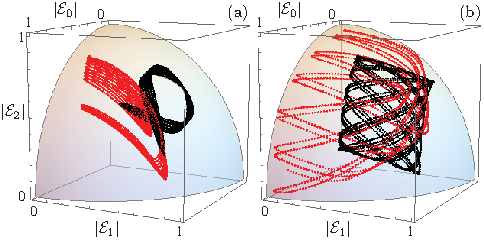
\includegraphics[width=\linewidth]{Fig2.pdf}}
\caption{(Color online) Absolute amplitude trajectories, $(\vert E_{0}(z) \vert, \vert E_{1}(z) \vert, \vert E_{2}(z) \vert )$, for initial random fields impinging random optical trimmers with constant parameters.}
\label{fig: Fig2}
\end{figure}

Dealing with the problem in the intensity-phase picture does not make it easier to solve but it provides insight.
Given a trimmer parameter set, $S(z) = \left\{ \omega_{j}(z), g_{jk}(z) \right\}$, and an initial field configuration, $\mathcal{E}(0) = \left\{ \mathcal{E}_{j}(0) \right\}$, it is possible to calculate the energy of the orbit, $H(0) = \epsilon\left(S(0), \mathcal{E(0)}\right)$. Then, it is possible to find the conditions that define the envelope of such orbit in the absolute value of the field amplitude plots via simultaneous minimization of $H(z) - \epsilon = 0 $,  $\partial_t n_j = 0$ and $\partial_t \phi_j = 0$ for $j= 0,1$.



%%%%%%%%%%%%%%%%%%%%%%%%%%%%%%%%%%%%%%%%%%%%%%%%%%%%%%%%%%%%%%%%%%%%%%%%%%%%%%%%%%%%%%%%%%%%%%%%%%%
% A short introduction to $SU(3)$ and the formal solution to the most general model
%%%%%%%%%%%%%%%%%%%%%%%%%%%%%%%%%%%%%%%%%%%%%%%%%%%%%%%%%%%%%%%%%%%%%%%%%%%%%%%%%%%%%%%%%%%%%%%%%%%




\section{Group theory and propagators}

Group theory, as an instrument to explore the underlying structure of mathematical models describing the physical world, brings a layer of abstraction into physics that allows deeper insight.
For example, unitary matrices of rank three, just like our mode-coupling matrix in Eq.(\ref{eq:hmlt}), are commonly characterized by the special unitary group $SU(3)$.
This group is a household name in physics that is often related to the work of Gell-Mann \cite{GellMann1961}.
Typically, the fundamental building blocks of this group are given by the well known Gell-Mann matrices, which provide a punctual description of the underlying algebraic structure.
Here, however, we will choose a different representation for the group \cite{Ticciati1999}, 
\begin{eqnarray}
\hat{I}_{0} = \frac{1}{2} \left( \begin{array}{ccc} 1&0&0\\0&-1&0\\0&0&0 \end{array}\right), \quad  
\hat{Y}_{0} = \frac{1}{3} \left( \begin{array}{ccc} 
1&0&0\\0&1&0\\0&0&-2    \end{array}\right), \nonumber\\
\hat{I}_{+} = \left( \begin{array}{ccc} 0&1&0\\0&0&0\\0&0&0 \end{array}\right), \quad 
\hat{I}_{-} = \left( \begin{array}{ccc} 0&0&0\\1&0&0\\0&0&0 \end{array}\right), \quad \nonumber\\
\hat{U}_{+} = \left( \begin{array}{ccc} 0&0&0\\0&0&1\\0&0&0 \end{array}\right), \quad 
\hat{U}_{-} = \left( \begin{array}{ccc} 0&0&0\\0&0&0\\0&1&0 \end{array}\right), \quad \nonumber \\
\hat{V}_{+} = \left( \begin{array}{ccc} 0&0&1\\0&0&0\\0&0&0 \end{array}\right), \quad 
\hat{V}_{-} = \left( \begin{array}{ccc} 0&0&0\\0&0&0\\1&0&0 \end{array}\right), \label{eq:gens}
\end{eqnarray}
due to the fact that we can understand matrices $\hat{I}_{\pm}$, $\hat{U}_{\pm}$ and $\hat{V}_{\pm}$ as those describing the coupling of the electromagnetic field between waveguides zero and one, one and two, and zero and two, in that order.
Thus, our mode-coupling matrix, in terms of the $SU(3)$ group, is given by the following expression,
\begin{eqnarray}
	\hat{H} &=& g_{01}(z) \left( \hat{I}_{+} + \hat{I}_{-} \right) + g_{12}(z) \left( \hat{U}_{+} + \hat{U}_{-} \right)\nonumber \\
	 & & +  g_{02}(z) \left( \hat{V}_{+} + \hat{V}_{-} \right).
\end{eqnarray}
The standard Wei-Norman technique for SU(3) is revisited in Ref. \cite{Dattoli1987p1582}, here we will show that the physical restrictions of the optical trimmer allows for further simplification.

Now, let us revisit the power of using underlying symmetries to evaluate propagation in arrays of coupled waveguides \cite{VillanuevaVergara2015p}. 
Any given normalized field vector that solves the Schr\"odinger-like mode coupling equation, Eq.(\ref{eq:diff}), 
\begin{eqnarray}
	\vert \mathcal{E}(z) \rangle = \hat{U}(z)  \vert 	\mathcal{E}(0) \rangle, \label{eq:sol}
\end{eqnarray}
can be written in terms of a $su(3)$ Lie algebra, in other words, the propagator is given by the following expression, 
\begin{eqnarray}
	\hat{U}(z) = \prod_{j=1}^{8} e^{i \theta_{j}(z) \hat{X}_{j}}.
\end{eqnarray}
where the algebra elements, $e^{i \theta_{j}(z) \hat{X}_{j}}$, are just the exponential map of the group generators, Eq.(\ref{eq:gens}), the functions $\theta_{j}(z)$ are complex functions ruled by the dynamics provided by the mode-coupling matrix, and the impinging field amplitudes are collected in the normalized initial field vector $\vert \mathcal{E}(0) \rangle$.

Note, there is no apriori ordering of $su(3)$ elements to write the propagator. 
However, the values of the prefixed $\theta_{j}(z)$ functions do depend on the chosen order.
We will choose a particular ordering,
\begin{eqnarray}
\hat{U}(z) &=& e^{i \iota_{+}(z) \hat{I}_{+}} e^{i \mu_{+}(z) \hat{U}_{+}}  
e^{i \nu_{+}(z) \hat{V}_{+}} e^{ \iota_{0}(z) \hat{I}_{0}} \nonumber \\ 
&& \times e^{i y_{0}(z) \hat{Y}}  e^{i \nu_{-}(z) \hat{V}_{-}} e^{i \mu_{-}(z) \hat{U}_{-}} e^{i \iota_{-}(z) \hat{I}_{-}}, \label{eq:prop}
\end{eqnarray}
that keeps us in line with the idea of understanding propagation through waveguide lattices as generalized Gilmore-Perelomov coherent states \cite{VillanuevaVergara2015p}.

Substituting the propagated field vector, Eq.(\ref{eq:sol}) considering as propagator Eq.(\ref{eq:prop}), into the mode coupling equation, Eq.(\ref{eq:diff}), is a cumbersome but straightforward operation that yields a set of eight coupled differential equations,
\begin{eqnarray}
	\iota_{+}^{\prime} &=& g_{01} \left( \iota_{+}^2 + 1 \right) + g_{12}  \iota_{+}  \nu_{+} - i  g_{03}   \nu_{+},    \label{eq:iota} \\
	\iota_{0}^{\prime} &=& i \left[ \left(- 2 g_{01} + i g_{02} \mu_{+}  \right) \iota_{+}  - g_{02} \nu_{+} + g_{12} \mu_{+} \right], \\
	\iota_{-}^{\prime} &=& e^{i \iota_0} \left( g_{1} - i g_{02}\mu_{+} \right), \\
	\mu_{+}^{\prime} &=& \left( - g_{01} + i  g_{02} \mu_{+} \right) \iota_{+} \mu_{+}    +  g_{12} \left( \mu_{+}^2 +  1 \right)\nonumber \\
	&&  +  \left( i  g_{01} + g_{02} \mu_{+} \right) \nu_{+},   \\
	\nu_{+}^{\prime} &=& g_{01} \iota_{+} 
	\nu_{+} + g_{02} (  \nu_{+} ^2
	+ 1)-i  g_{12} \iota_{+}, \label{eq:mu} \\
	y_{0}^{\prime} &=& -i\frac{3}{2}  
	[ g_{02}   \nu_{+}+  \mu_{+}  
	( g_{12}+i  g_{02} \iota_{+})],  \\
	\nu_{-}^{\prime} &=& e^{\frac{1}{2}i(2y_0+\iota_0)}
	g_{02} +i e^{i\iota_{0}}  \mu_{-}  (i g_{02} 
	 \mu_{+}-  g_{01}),  \\
	\mu_{-}^{\prime} &=&  e^{i y_0-\frac{1}{2}i \iota_0}
	( g_{12}+i  g_{02} \iota_{+}), 
\end{eqnarray}
where, for the sake of space, we have used $f \equiv f(z)$ and $f' \equiv \partial_{z} f(z)$ for all propagation dependent auxiliary functions and couplings.

Non-linear differential equations are known to be hard to solve and finding a solution 
often requires intuition and knowledge of the system being analyzed. 
Before delving into details, we would like to point out a key feature of the present model, $\hat{H}^{T}(z) = \hat{H}(z)$, that is, the mode-coupling matrix is symmetric, and, as a direct consequence, the propagator shares the same property,
\begin{equation}  
	\hat{U}^{T}(z)=\hat{U}(z).
\end{equation} 
This feature allows us to conclude that the propagator functions are symmetric,
\begin{eqnarray}
	\iota_{+}(z)&=&\iota_{-}(z) \label{eq:sym1}\\
	\mu_{+}(z)&=&\mu_{-}(z)\\
	\nu_{+}(z)&=&\nu_{-}(z) . \label{eq:sym3}
\end{eqnarray}
Furthermore, we observe that two equations, namely Eq.(\ref{eq:iota}) and Eq.(\ref{eq:mu}) only include terms of $\iota_{+}(z)$ and $\nu_{+}(z)$ and their derivatives. 
Therefore, they are decoupled from the rest. 
Nonetheless, these two equations prove intractable and we will pursue a different route to finding a solution.
For reasons that will become apparent in a moment, we introduce a set of five auxiliary functions,
\begin{eqnarray}
	\Gamma(z) &=& e^{-\frac{3}{2} i y_{0}(z)} \\
	\Delta(z)&=& i e^{-\frac{3}{2} i y_{0}(z)} \mu_{\pm}(z) \\
	   \Theta(z)&=& e^{-\frac{2}{3}i y_0(z)} (-\iota_{\pm}(z) \mu_{\pm}(z) + i \nu_{\pm}(z)) \\
	\Pi(z)&=& e^{-\frac{2}{3} i y_{0} (z)}
	    (e^{i y_0 (z)-\frac{1}{2} i \iota_0 (z)}
		-\mu_{\pm} (z)^2) \\
	\Sigma(z)&=& e^{-\frac{2}{3} i y_0(z)} (i \iota_{\pm}(z) \Pi(z)-\mu_{\pm} (z) \nu_{\pm}(z))
\end{eqnarray}
These equations can be further decoupled,
\begin{eqnarray}
	\left( \begin{array}{c}
		\Theta^{\prime}(z) \\
	\Delta^{\prime}(z) \\
	\Gamma^{\prime}(z) 
		\end{array} \right)=iH 
		\left( \begin{array}{c}
	\Theta(z) \\
	\Delta(z) \\
		\Gamma(z) 
	\end{array} \right) \label{eq:set1}\\
	\left( \begin{array}{c}
	\Sigma^{\prime}(z) \\
	\Pi^{\prime} (z) \\
	\Delta^{\prime}(z) 
	\end{array} \right)=iH 
	\left( \begin{array}{c}
	\Sigma(z) \label{eq:set2}\\
	\Pi (z) \\
	\Delta(z)  
	\end{array} \right)
	\end{eqnarray}
via the identity, 
\begin{eqnarray}
g_{01}(z)\Theta(z) + g_{12}(z) \Gamma(z) =  g_{02}(z) \Sigma (z) + g_{12}(z) \Pi (z),
\end{eqnarray}
which is a direct consequence of $\mu_{+}(z)=\mu_{-}(z)$.
These two sets of differential equations can be readily solved with an additional set of initial values,
\begin{eqnarray}
\Theta(z)&=& 0 , \quad \Delta(z) =  0, \quad \Sigma(z)= 0,   \label{eq:initsa} \\
\Gamma(z)&=& 1, \quad \Pi(z)= 1. \label{eq:initsb}
\end{eqnarray}



The two coupled differential sets, Eq. (\ref{eq:set1}) and Eq.(\ref{eq:set2}), in conjunction the initial values, Eq. (\ref{eq:initsa}) and Eq.(\ref{eq:initsb}), 
unequivocally determine the five auxiliary functions that return, 
\begin{eqnarray}
\mu_{\pm}(z) &=& \frac{-i \Delta(z)}{\Gamma(z)} \\
\iota_{\pm}(z) &=& \frac{i(-\Gamma(z)\Sigma(z)+\Delta(z)\Theta(z))}{\Delta(z)^2-\Gamma(z)\Pi(z)}\\
\nu_{\pm}(z) &=& \frac{-i(\Delta(z)\Sigma(\zeta)-\Pi(z)\Theta(z))}{\Delta(z)^2-\Gamma(z)\Pi(z)}\\
y_0(z) &=&  \dfrac{3}{2} i \log (\Gamma(z))\label{eq:yzeto}\\
\iota_0(z) &=& 2 i \log (\frac{\Gamma(z)\Pi(z)-\Delta(z)^2}{\sqrt{\Gamma(z)}}) \label{eq:izero}
\end{eqnarray}
Note that the phase functions $y_0(z)$ and $i_0(z)$ are of logarithmical nature and the rest are quotients of the products of the solution basis. 

%%%%%%%%%%%%%%%%%%%%%%%%%%%%%%%%%%%%%%%%%%%%%%%%%%%%%%%%%%%%%%%%%%%%%%%%%%%%%%%%%%%%%%%%%%%%%%%%%%%
% Case of constant couplings
%%%%%%%%%%%%%%%%%%%%%%%%%%%%%%%%%%%%%%%%%%%%%%%%%%%%%%%%%%%%%%%%%%%%%%%%%%%%%%%%%%%%%%%%%%%%%%%%%%%

\subsection{Trimer with constant couplings}

While we have provided a formal solution to propagation through the optical trimer, considering a specific solution may help build further intuition. 
Thus, in this section, we will discuss the special case where all the couplings are independent of the propagation distance.
For the sake of simplicity, we will introduce the dimensionless propagation parameter $\zeta = g_{01} z$, such that the mode-coupling differential equation becomes 
\begin{eqnarray}
- i \partial_{\zeta} \vert \mathcal{E}(\zeta) \rangle = \hat{H} \vert \mathcal{E}(\zeta) \rangle, 
\end{eqnarray}
with the mode-coupling matrix,
\begin{eqnarray}
\hat{H} = \left( \begin{array}{ccc} 
0  & 1 & \alpha  \\
1 & 0 & \beta \\
\alpha & \beta & 0
\end{array} \right), \label{eq:hmlt2}
\end{eqnarray}
given in terms of the dimensionless parameters,
\begin{eqnarray}
\alpha =\frac{g_{02}}{g_{01}}, \quad \beta=\frac{g_{12}}{g_{01}}.
\end{eqnarray}
Under this constant mode-coupling matrix, we could use the results presented in the past section to build a particular solution, but it is well known that a set of linear first order differential equations is equivalent to a single linear differential equation of higher order.
It seems worthwhile deriving such an higher order differential equation for $\Delta(\zeta)$, which is the auxiliary function that connects the two sets of differential equations, Eq.(\ref{eq:set1}) and Eq.(\ref{eq:set2}).
After some algebra, it is possible to write,
\begin{equation}
\Delta^{\prime\prime\prime}(\zeta) + i(1+\alpha^2+\beta^2)\Delta ^{\prime}(\zeta) -2 \alpha\beta\Delta(\zeta) = 0,\label{eq:ddiff}
\end{equation}
with initial values,
\begin{eqnarray}
\Delta(0) & = & 0, \\
\Delta^{\prime}(0) &=& i\beta, \\
\Delta^{\prime\prime}(0) &=& -\alpha.
\end{eqnarray}
It is easy to see that $\Delta(\zeta)$ has the following solution,
\begin{eqnarray}
\Delta(\zeta) = \delta_{1} \: e^{i \gamma_1 \zeta} + \delta_{2} \: e^{i \gamma_2 \zeta} +  \delta_{3} \: e^{i \gamma_3 \zeta},
\end{eqnarray}  
where constant parameters  $\gamma_{j}$ are the eigenvalues of the mode-coupling matrix determined by the characteristic polynomial, a reduced cubic,
\begin{eqnarray}
\gamma_{j}^{3} - (1+ \alpha^{2} + \beta^{2}) \gamma_{j} - 2 \alpha \beta = 0. \label{eq:poly}
\end{eqnarray}
It is straightforward to notice that there are three different real eigenvalues for real, positive, non-zero coupling parameters, $\alpha, \beta > 0$.
These proper values can be writen in a closed but non-compact form, so we will not write them explicitly.
Furthermore, the coefficients are given by
\begin{eqnarray}
\delta_{1} &=& \frac{\alpha-\beta(\gamma_2+\gamma_3)}{(\gamma_1-\gamma_2)(\gamma_1-\gamma_3)},\\
\delta_{2} &=& \frac{\alpha-\beta(\gamma_1+\gamma_3)}{(\gamma_2-\gamma_1)(\gamma_2-\gamma_3)},\\
\delta_{3} &=& \frac{\alpha-\beta(\gamma_1+\gamma_2)}{(\gamma_3-\gamma_1)(\gamma_3-\gamma_2)}. 
\end{eqnarray}  
The remaining auxiliary functions are straightforward to calculate, 
\begin{eqnarray}
\Theta(\zeta)&=& \frac{\beta(1+\beta^2)\Delta(\zeta) - i \alpha\Delta^{\prime}(\zeta)+\beta\Delta^{\prime\prime}(\zeta)}
	{\alpha(1-\beta^2)}  \\
\Gamma(\zeta)&=& \frac{-(1+\beta^2)\Delta(\zeta) +i \alpha\beta\Delta^{\prime}(\zeta)-\Delta^{\prime\prime}(\zeta)}
	{\alpha(1-\beta^2)} \\
\Sigma(\zeta)&=& \frac{\beta(\alpha^2+\beta^2)\Delta(\zeta) -i \alpha\Delta^{\prime}(\zeta)+\beta\Delta^{\prime\prime}(\zeta)}
	{\alpha^2-\beta^2}  \\
\Pi(\zeta)&=& \frac{-\alpha(\alpha^2+\beta^2)\Delta(\zeta) +i \beta\Delta^{\prime}(\zeta)-\alpha\Delta^{\prime\prime}(\zeta)}
	{\alpha^2-\beta^2}.
\end{eqnarray} 
Thus, the propagator functions, $\iota_{\pm}(z)$, $\mu_{\pm}(z)$, $\nu_{\pm}(z)$, $\iota_{0}(z)$ and $y_{0}(z)$, will effectively contain terms involving the three eigenvalues as well as sums and differences thereof.


%%%%%%%%%%%%%%%%%%%%%%%%%%%%%%%%%%%%%%%%%%%%%%%%%%%%%%%%%%%%%%%%%%%%%%%%%%%%%%%%%%%%%%%%%%%%%%%%%%%
% Practical examples
%%%%%%%%%%%%%%%%%%%%%%%%%%%%%%%%%%%%%%%%%%%%%%%%%%%%%%%%%%%%%%%%%%%%%%%%%%%%%%%%%%%%%%%%%%%%%%%%%%%

\section{Applications}

Let us present some practical examples of optical trimers that may have a feasible experimental realization.


\subsection{Identical couplings and the discrete Fourier transform}

The mode-coupling matrix for three-identical waveguides distributed in an equilateral triangle configuration, $\alpha = \beta = 1$, 
\begin{equation}
\hat{H}=\left( \begin{array}{ccc}
0 & 1 & 1 \\
1 & 0 & 1 \\
1 & 1 & 0 \end{array} \right),	 
\end{equation}
is related to the cyclic group in dimension three, 
\begin{eqnarray}
\hat{H} =  \hat{Z}_{3} + \hat{Z}_{3}^{2} ,
\end{eqnarray}
where the generator of the cyclic group, 
\begin{eqnarray}
\hat{Z}_{3} &=& \hat{I}_{+} + \hat{U}_{+} + \hat{V}_{-}, \nonumber \\
&=&\left(
\begin{array}{ccc}
 0 & 1 & 0 \\
 0 & 0 & 1 \\
 1 & 0 & 0 \\
\end{array}\right).
\end{eqnarray}
It is well known that the cyclic group is diagonalized by the discrete Fourier transform, $\hat{\Lambda} = \hat{F}_{n} \hat{Z}_{n} \hat{F}_{n}^{\dagger}$, where the discrete Fourier transform of rank $n$ is given by the operator $\hat{F}_{n}$,  in the case of $n=3$,
\begin{eqnarray}
\hat{F}_{3} &=& 
\frac{1}{\sqrt{3}}
\left(
\begin{array}{ccc}
 1 & 1 & 1 \\
 1 & e^{\frac{2 i \pi}{3}} & e^{-\frac{2 i \pi}{3}} \\
 1 & e^{-\frac{2 i \pi}{3}} & e^{\frac{2 i \pi}{3}} \\
\end{array}\right),
\end{eqnarray}
and $\hat{\Lambda}$ is a diagonal rank $n$ matrix containing the roots of unity, $\hat{\Lambda}_{mn} = \delta_{m,n} e^{ i \frac{2 \pi}{n} i}$ with $m,n = 0,1,2$.
In this particular case, it is possible to compose a propagator,
\begin{eqnarray}
U(\zeta) &=& \hat{F}_{3}^{\dagger} e^{i \hat{\Lambda}_{3} \zeta} e^{i \hat{\Lambda}_{3}^{2} \zeta} \hat{F}_{3}, \nonumber \\
&=& \frac{1}{3}\left(
\begin{array}{ccc}
 2+e^{3 i \zeta} & -1+e^{3 i \zeta} & -1+e^{3 i \zeta} \\
 -1+e^{3 i \zeta} & 2+e^{3 i \zeta} & -1+e^{3 i \zeta} \\
 -1+e^{3 i \zeta} & -1+e^{3 i \zeta} & 2+e^{3 i \zeta} \\
\end{array}
\right) e^{-i \zeta},
\end{eqnarray}
where we have used the fact that the elements of the cyclic group of rank $3$ commute between them, $\left[ \hat{Z}_{3} , \hat{Z}_{3}^{2} \right] = 0$ because $\hat{Z}_{3}^{3} = \mathbb{1}_{3}$.  

Figure \ref{fig: Fig3} shows the trajectories described by the absolute value of the field amplitudes, $\vert \mathcal{E}_{j}(z)\vert$, as they propagate. 
All of trajectories will lie over the surface of an octant of the sphere due to unitary propagation.
Figure \ref{fig: Fig3}(a) shows the response to impulses, $\mathcal{E}_{j} = \delta_{j,k}$ with $j=0,1,2$ and a fixed $k=0,1,2$. 
Figure \ref{fig: Fig3}(b) shows the trajectories given by initial field superpositions of the more general form: $\mathcal{E}_{j} = \alpha_{j} e^{i \phi t}$ with $\alpha \in \mathbb{R}$ and $\sum_{j} \vert \alpha_{j} \vert^{2} =1$.
From the propagator, it is possible to see that only two commensurate frequencies are involved in the propagation of initial fields, thus, the trajectories will be closed and well defined.


\begin{figure}[htbp]
\centering
\fbox{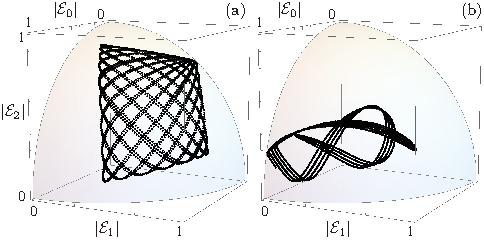
\includegraphics[width=\linewidth]{Fig3.pdf}}
\caption{(Color online) Absolute amplitude trajectories, $(\vert E_{0}(z) \vert, \vert E_{1}(z) \vert, \vert E_{2}(z) \vert )$, for initial fields, $(\vert E_{0}(0) \vert, \vert E_{1}(0) \vert, \vert E_{2}(0) \vert )$, impinging (a) only the zeroth (black), $(1,0,0)$, first (blue), $(0,1,0)$, and second (red), $(0,0,1)$, waveguides and (b) initial fields impinging two waveguides at a time with and without a relative phase, $(\frac{1}{\sqrt{2}},\frac{1}{\sqrt{2}},0)$ (black), $(\frac{1}{\sqrt{2}},\frac{i}{\sqrt{2}},0)$ (blue), and $(\frac{2}{\sqrt{5}},0,\frac{i}{\sqrt{5}})$ (red).}
\label{fig: Fig3}
\end{figure}




\subsection{Two identical couplings and the golden ratio}
In the case of two equal coupling parameters the unitless Hamiltonian becomes
\begin{equation}
H=\left( \begin{array}{ccc}
0 & 1 & \alpha \\
1 & 0 & \alpha \\
\alpha & \alpha & 0 \end{array} \right)	 
\end{equation}
Note that the Hamiltonian is  $\hat{Z}_2$-invariante, i.e. it is invariant under xchanging the first and the second waveguide.
This symmetry also is reflected by the eigenvalues which are  $\left\{-1, \bar{\varphi}, \varphi  \right\}$ with
\begin{eqnarray}
\bar{\varphi} &=& \frac{1}{2} \left(1-\sqrt{8 \alpha ^2+1}\right),\\
\varphi &=& \frac{1}{2} \left( 1 + \sqrt{8 \alpha ^2+1} \right).
\end{eqnarray}
It is simple to see that $\bar{\varphi} + \varphi = 1$ and the second and third eigenvalue do transform into 
each other upon applying the complex conjugate. Note that the latter eigenvalue 
assumes the golden ratio for $\alpha = \sqrt{1/2}$.
Due to the $\hat{Z}_2$-symmetry the propagator can be calculated directly from the Hamiltonian and can be written as:
\begin{eqnarray}
U(\zeta) = \frac{1}{\varphi -\bar{\varphi}} \left(
\begin{array}{ccc}
f(\zeta) & g(\zeta) &  h(\zeta)\\
g(\zeta) & f(\zeta) & h(\zeta) \\
h(\zeta) & h(\zeta) & i(\zeta) \\
\end{array}
\right)\label{eq:prop2}
\end{eqnarray}
 with
 \begin{eqnarray}
f(\zeta) &=& \frac{\varphi}{2} e^{i \zeta \varphi} -\frac{\bar{\varphi}}{2} e^{i \zeta \bar{\varphi} }
 + \frac{1}{2} \left( \varphi -\bar{\varphi} \right) e^{-i \zeta}, \label{eq:ticF1}\\
g(\zeta) &=& \frac{\varphi}{2} e^{i \zeta \varphi } - \frac{\bar{\varphi}}{2} e^{i \zeta \bar{\varphi} } - \frac{1}{2} \left( \varphi -\bar{\varphi}\right)  e^{-i \zeta}, \\
h(\zeta) &=& \alpha \left(  e^{i \zeta \varphi }  -  e^{i \zeta \bar{\varphi} } \right),\\
i(\zeta) &=&   \varphi e^{i \zeta \bar{\varphi} } - \bar{\varphi}  e^{i \zeta \varphi } \label{eq:ticF2} 
\end{eqnarray}
In operator form the propagator yields
\begin{eqnarray}
U(\zeta)=\frac{g(\zeta)}{\varphi -\bar{\varphi}}\;(I_{+}+I_{-})
+\frac{h(\zeta)}{\varphi -\bar{\varphi}}\;(U_{+}+U_{-}+V_{+}+V_{-})
\nonumber\\
+\frac{2}{3}\frac{f(\zeta)-i(\zeta)}{\varphi -\bar{\varphi}}\;(U_{0}+V_{0})  
+\frac{1}{3}\frac{i(\zeta)+2f(\zeta)}{\varphi -\bar{\varphi}}\;\mathbbm{1}
\end{eqnarray}
\newline
Obviously the three eigenvalues are stationary point of the system. 
However,the particular symmetry of the system might allow for further
interesting states. \newline
Looking at the propagator functions (\ref{eq:ticF1}) to (\ref{eq:ticF2}) reveals that 
two of the equations, namely $h(\zeta)$ and $i(\zeta)$ depend on only two of the three
eigenfrequencies, $\varphi$ and $\bar{\varphi}$. Equation (\ref{eq:prop2}) further reveals that the 
evolution of the third component only depends on those two equations $h(\zeta)$ and $i(\zeta)$.
Now one can hope that if we chose the initial eigenstate accordingly one of the two 
eigenfrequencies in the evolution of the third component will cancel out. That is, if
the evolution only depends on one frequency, it will only change in phase and the 
amplitude will remain immutable. \newline
Hence, lets look for such a state where no energy transfer into or out of the third component occurs. Without loss of 
generality we can assume that the state-vector at a given time bears following form:
\begin{equation}
\mathcal{E}(\zeta=0)=\left( \begin{array}{c}
0 \\
\mathcal{E}_2(0) \\
\mathcal{E}_3(0)
\end{array} \right)	
\end{equation}   
Which implies that the third component evolves as:
\begin{equation}
(\varphi -\bar{\varphi})\mathcal{E}_3(\zeta) = h(\zeta)\mathcal{E}_2(0)
+i(\zeta)\mathcal{E}_3(0)
\end{equation}
As argued above the third waveguide will not change in amplitude if one of the 
two eigenfrequencies cancel out. This is fulfilled if either of the two following conditions
is met:
\begin{eqnarray}
\mathcal{E}_2(0)=\mathcal{E}_3(0)\frac{\varphi}{\alpha}\quad or \quad
\mathcal{E}_2(0)=\mathcal{E}_3(0)\frac{\bar{\varphi}}{\alpha}
\end{eqnarray}
Consequently we obtain two solutions for a state with stationary amplitude in the third waveguide.
 Without loss of generality we can normalise the initial state such that the amplitude of the third component is one, ie $\mathcal{E}_3(0)=1$.
 Then the time evolution of the system is given by:
\begin{equation}
\mathcal{E}_{\varphi}(\zeta)=\left( \begin{array}{c}
\frac{g(\zeta)}{\varphi -\bar{\varphi}}\frac{\varphi}{\alpha}+\frac{h(\zeta)}{\varphi -\bar{\varphi}} \\
\frac{f(\zeta)}{\varphi -\bar{\varphi}}\frac{\varphi}{\alpha}+\frac{h(\zeta)}{\varphi -\bar{\varphi}} \\
e^{i\zeta\varphi}
\end{array} \right)	
\end{equation}
and
\begin{equation}
\mathcal{E}_{\bar{\varphi}}(\zeta)=\left( \begin{array}{c}
\frac{g(\zeta)}{\varphi -\bar{\varphi}}\frac{\bar{\varphi}}{\alpha}+\frac{h(\zeta)}{\varphi -\bar{\varphi}} \\
\frac{f(\zeta)}{\varphi -\bar{\varphi}}\frac{\bar{\varphi}}{\alpha}+\frac{h(\zeta)}{\varphi -\bar{\varphi}} \\
e^{i\zeta\bar{\varphi}}
\end{array} \right)	
\end{equation}




\section{Conclusion}
We have shown that it is possible to solve the light evolution
equations in a coupled three-core waveguide, in terms of
the Lie group generators of su(3). We focused our attention on a
reduced class of structures where the coupling constants
are constant in position......... As an
example we consider the case of equal coupling constants.
we found that the dynamics of such a system i 
governed by a linear third order differential equation and the
corresponding five auxiliary functions can be expressed in term of its solution.
we also established a connection between a waveguide cluster
with equal couplings and the well known Fourier transform, possibly opening
a path to realise quantum Fourier transformations.
furthermore we studies an isosceles waveguide triangle.
We showed that two equal couplings corresponds to
a Z2 symmetry of the Hamiltonian. We also showed 
that the symmetry allows for two interesting stated
characterised by absence of energy transfer into the 
third core.


%\section*{Funding Information}

%\textbf{Funding.} 

%\section*{Acknowledgments}

%\textbf{Acknowledgment.} 


%\section*{References}
% Bibliography
\bibliographystyle{osajnl}
\bibliography{D:/ExternalHD/Bibliography/references}


\end{document}

\section{Trimer with two identical couplings}

If we ease the general problem and allow two couplings to be equal, $g_{02}(z) = g_{12}(z) = g(z)$, it seems worthwhile trying to find a higher order differential equation for $\Delta(\zeta)$, which is the auxiliary function that connects the two sets of differential equations, Eq.(\ref{eq:set1}) and Eq.(\ref{eq:set2}).
After some algebra, it is possible to write,
\begin{equation}
\Delta^{\prime \prime}(\zeta) - \left[ i g_{01}(z) + \frac{g^{\prime}(z)}{g(z)} \right]  \Delta^{\prime}(\zeta) + 2 g^{2}(z) \Delta(\zeta) = 0,\label{eq:ddiff}
\end{equation}
with initial values,
\begin{eqnarray}
\Delta(0) & = & 0 , \\
\Delta^{\prime}(0) &=& i g(0). 
\end{eqnarray}
In this case, the remaining auxiliary functions are given by the following expressions,

For example, the case of a constant coupling, $g_{01}$, and two sinusoidal coupling functions, 
\begin{eqnarray}
g(z) = g_{01} \left[ 1 + \alpha \sin \left( k z \right) \right], \quad \vert \alpha \vert < 1,
\end{eqnarray}
